\documentclass{beamer}
\title{Wegfindung im Labyrinth (AP)}
\author{\texorpdfstring{Florian Nowak \& Yichuan Shen\\ Betreuer: Gero Plettenberg, Thomas Kloepfer}{Florian Nowak \& Yichuan Shen}}
\date{Wintersemester 2014/15}

%\usetheme{Goettingen}
\setbeamertemplate{navigation symbols}{}

\usepackage[utf8]{inputenc}

\usepackage[ngerman]{babel}
%\usepackage{lmodern}
\usepackage[default]{sourcesanspro}

\usepackage{float,graphicx,subfig}
  \graphicspath{{bilder/}}

\usepackage{tikz}
  \usetikzlibrary{shapes}
  \tikzstyle{every picture} += [font=\sffamily]

\usepackage{xparse}
  \NewDocumentCommand\blocking{m}{\textcolor{green}{\textit{#1}}}
  \NewDocumentCommand\blue{m}{{%
  	\usebeamercolor[fg]{frametitle}{#1}%
  }}
  \NewDocumentCommand\longunderscore{}{%
  	\underline{\hphantom{\textunderscore\textunderscore}}%
  }
  
\usepackage{minted}
  \usemintedstyle{monokai}
  

\begin{document}
\maketitle

\tikzstyle{startend}=[
  circle,
  text centered,
  very thick,
  draw=red!50!black!70,
  fill=red!50!black!30,
  %top color=white,
  %bottom color=red!50!black!30
  ]
\tikzstyle{rounded}=[
  rounded rectangle,
  text centered,
  very thick,
  draw=lime!50!black!70,
  fill=lime!50!black!30,
  %top color=white,
  %bottom color=lime!50!black!30
  ]
\tikzstyle{kugel}=[
  rounded rectangle,
  text centered,
  text width=2.25cm,
  very thick,
  draw=blue!50!black!70,
  fill=blue!50!black!30,
  %top color=white,
  %bottom color=blue!50!black!30
  ]
\tikzstyle{block}=[
  rectangle,
  text centered,
  %text width=1cm,
  very thick,
  draw=black!40,
  fill=black!24,
  %top color=white,
  %bottom color=black!30
  ]
\tikzstyle{decision}=[
  diamond,
  text centered,
  %text width=1cm,
  very thick,
  draw=lime!50!black!70,
  fill=lime!50!black!30,
  %top color=white,
  %bottom color=lime!50!black!30
  ]
\tikzstyle{line}=[draw, thick, ->]

\begin{frame}[fragile,t]{Gegeben}
\begin{center}
\includegraphics[scale=.13]{roboter_no-maze}
\end{center}
\begin{itemize}
\item Ein Roboter mit neigbarem Touchscreen und einer Metallkugel
\item Die Position der Kugel kann bestimmt werden.
\item Die Kugel kann in einer vorgegebener Richtung gelenkt und zum Stillstehen gebracht (balanciert) werden.
\end{itemize}
\end{frame}

\begin{frame}[fragile,t]{Aufgabenstellung}
\begin{center}
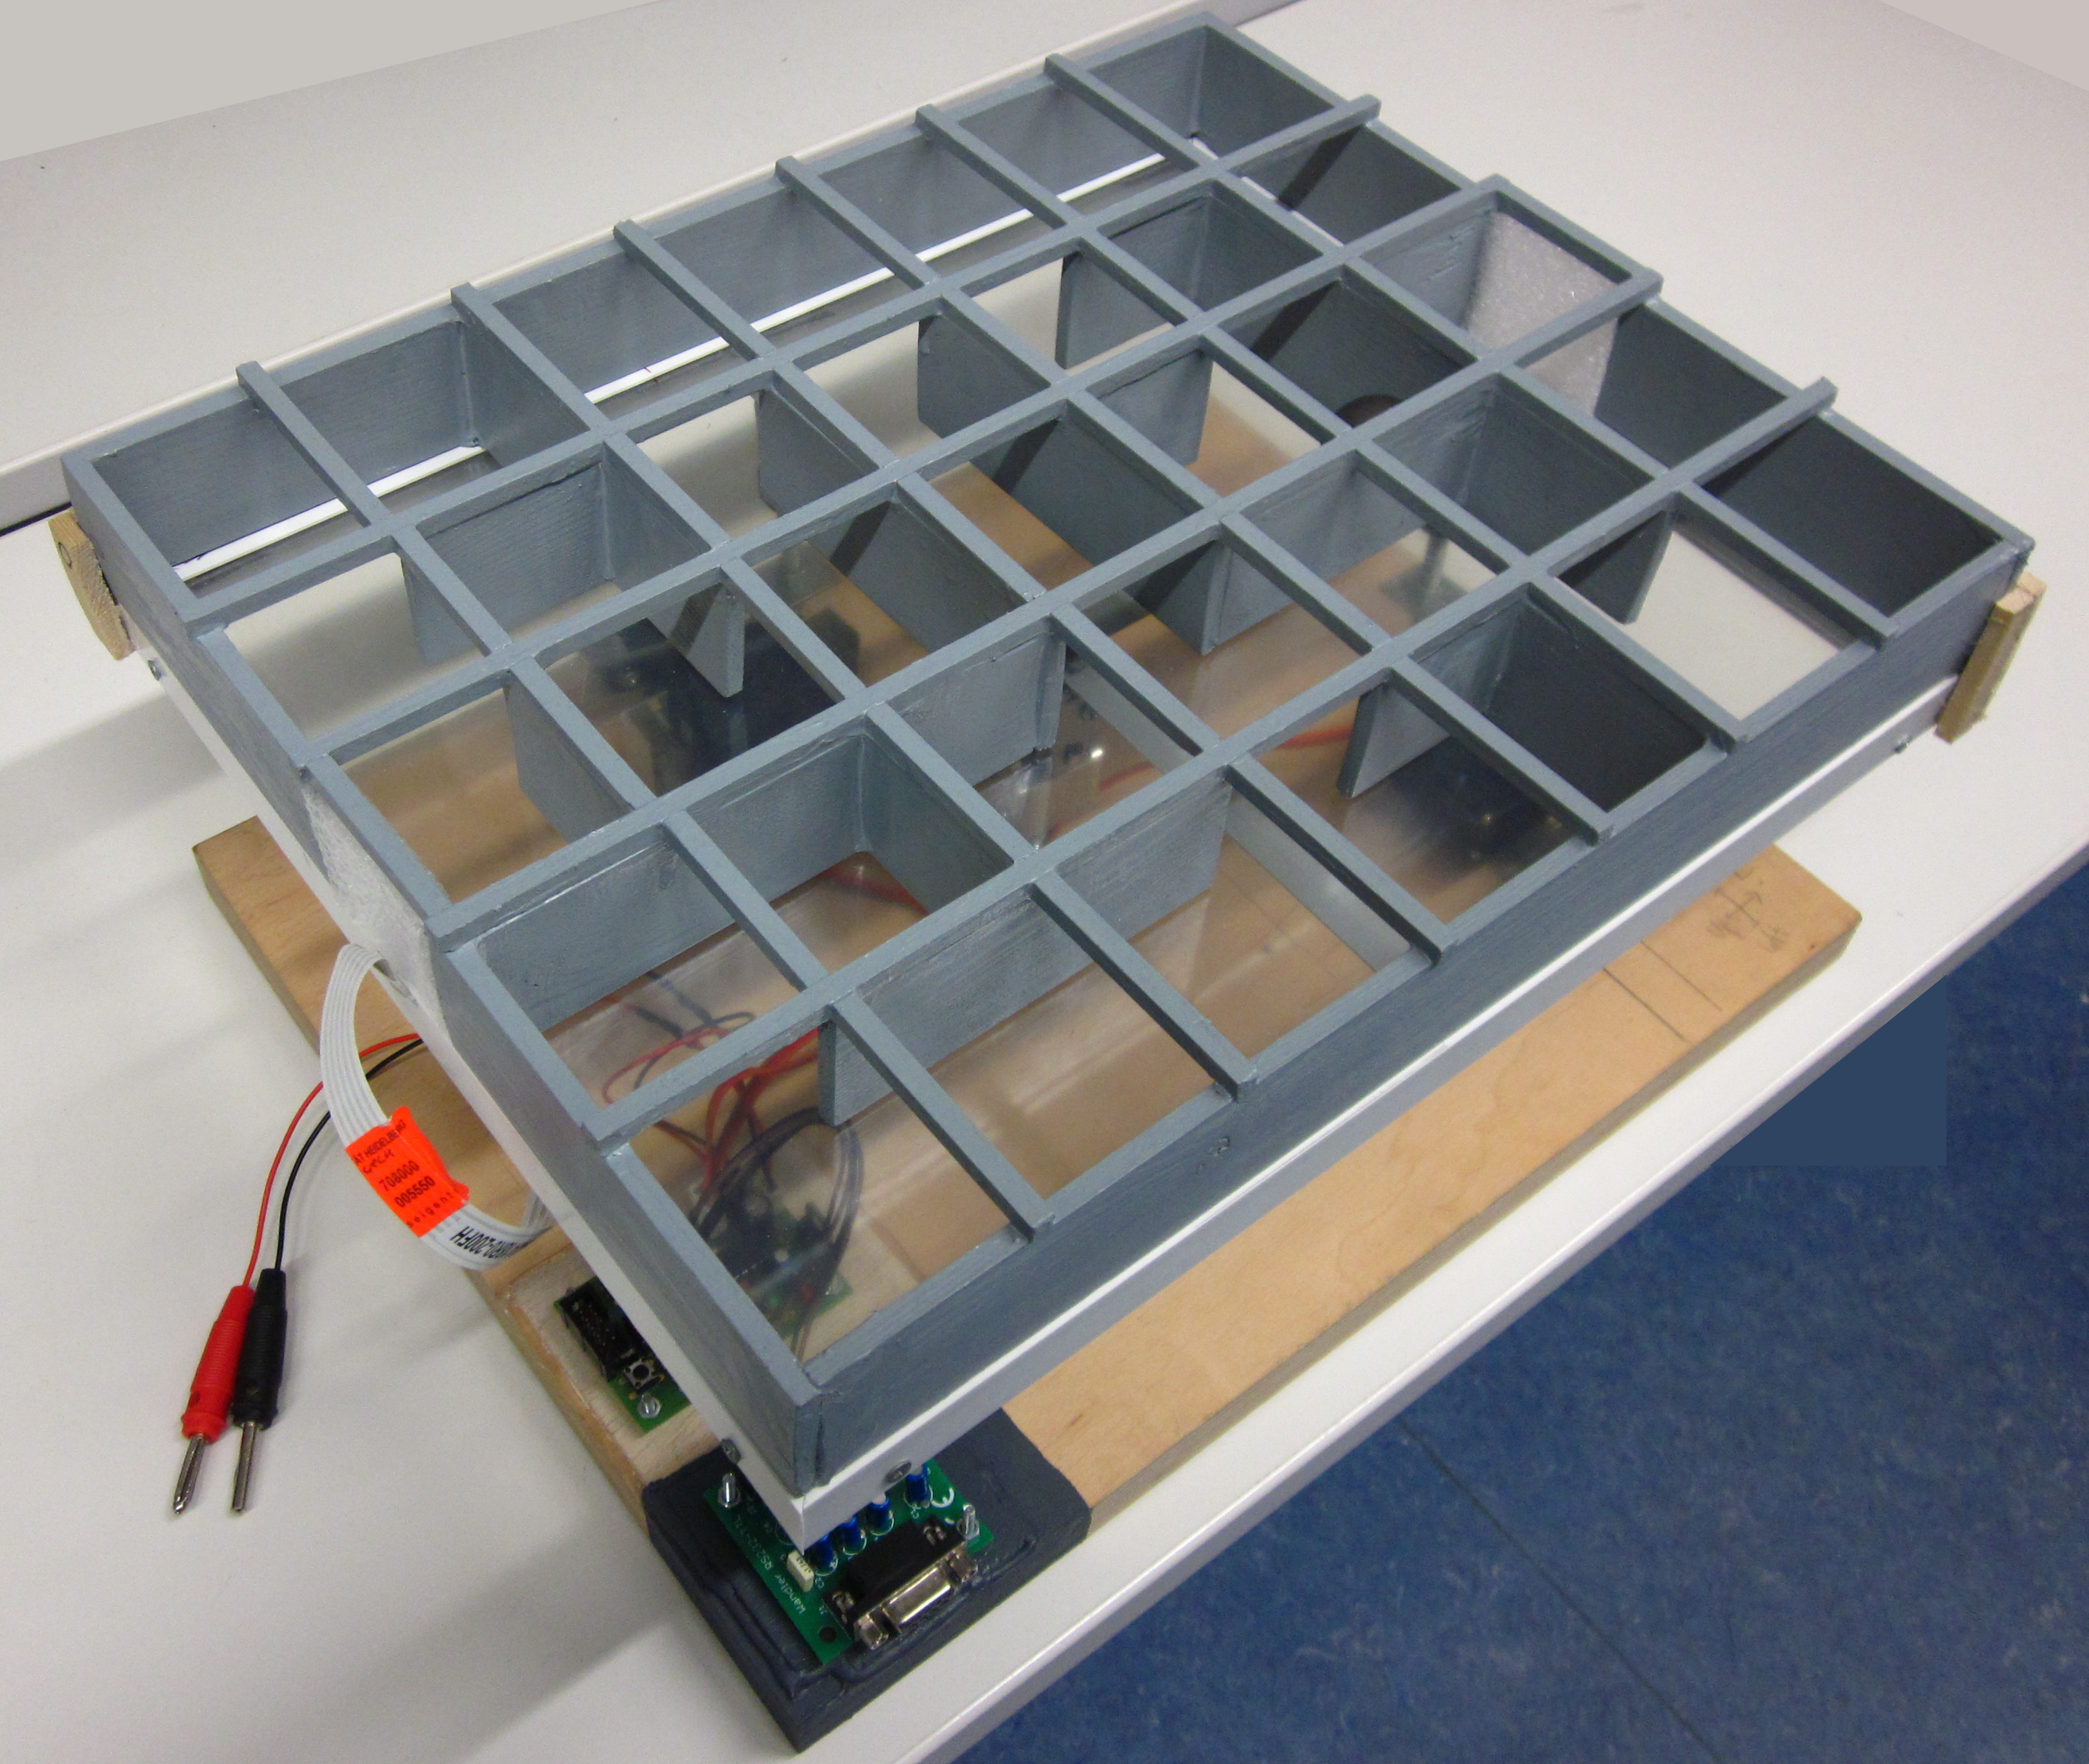
\includegraphics[scale=.12]{roboter_badly-photoshoped}
\end{center}
\begin{itemize}
\item Die Struktur eines beliebiges, auf dem Touchscreen liegendes Labyrinth soll eingelesen werden.
\item Die Kugel soll ein zuvor eingelesenes Labyrinth optimal durchlaufen können.
\end{itemize}
\end{frame}

\iffalse
\begin{frame}[fragile,t]{Aufgabenstellung}
Ein bereits vorhandener Roboter mit neigbarem Touchscreen soll etwas Neues lernen: Er soll ein beliebiges auf dem Rahmen seines Touchscreens aufliegendes Labyrinth (vorgegebener Rastergröße) mithilfe einer Metallkugel einlesen können. Der Roboter kann eine solche Kugel bereits auf eine ihm vorgegebene Position durch Kippen rollen lassen (und dort auch zum Stillstehen bringen). Das Ziel ist es somit, den Roboter ein zuvor eingelesenes Labyrinth mit der Kugel (auf optimalem Weg) lösen zu lassen.

\medskip\noindent
\blocking{Aufgabenstellung am Roboter erläutern!}
\end{frame}
\fi

\begin{frame}[fragile,t]{Vorstellung}
\blocking{Kurz vorstellen!}
\end{frame}

\begin{frame}[fragile,t]{Demonstration}
\blocking{\verb~string~-Darstellung des vorhandenen Labyrinths einlesen und Labyrinth lösen! Anschließend mit der Tiefensuche beginnen!}
\end{frame}

\begin{frame}[fragile,t]{Praktikumsverlauf}{Milestones}
\begin{enumerate}
 \item \blue{Einarbeitung} \textit{(bis Anfang Dezember)}\blue{:}\\
 Vorgängercode und Funktionsfähigkeit des Roboters testen.
 \item \blue{Durchlaufen des Labyrinths} \textit{(bis Anfang Januar)}\blue{:}\\
 Durch Vorgabe eines Labyrinths als Datenstruktur soll die Kugel einen beliebig vorgegebenen Pfad durchlaufen können. Ferner wird ein optimaler Weg durch das Labyrinth berechnet.
 \item \blue{Erkennen des Labyrinths} \textit{(bis Ende Januar)}\blue{:}\\
 Durch Ablaufen eines realen Labyrinths soll die Struktur des Labyrinths erkannt und abgespeichert werden. Dafür wird ein Algorithmus entworfen und implementiert.
 \textcolor{gray}{
 \item[\textcolor{gray}{4.}] Fertigstellung \textit{(bis Anfang März)}:\\
Präsentation, Poster und Webseite fertig stellen; ggf. eine grafische Oberfläche erstellen.
}
\end{enumerate}
\end{frame}

\begin{frame}[fragile,t]{Praktikumsverlauf}
\begin{itemize}
\item Zeitplan konnte recht gut einhalten werden
\item Milestone 3 ist wie erwartet aufwendiger geworden:

\begin{enumerate}
 \item[3.] \blue{Erkennen des Labyrinths (Tiefensuche)}
 \begin{enumerate}
 \item[(a)] Entwurf einer Routine zur Wanderkennung
 \item[(b)] Optimierung (hinsichtlich Geschwindigkeit)
 \end{enumerate}
 \item[\textcolor{gray}{4.}] \textcolor{gray}{Fertigstellung}
\end{enumerate}
\item Hinzugekommen sind (optische) Verbesserungen an der Hardware\\
\blocking{Am Roboter zeigen!}
\end{itemize}
\end{frame}

\begin{frame}[fragile,t]{Herangehensweise an die Problemstellung}
\begin{itemize}
\item Festlegung von \blue{Python (2.7)} als Programmiersprache
\item Auswahl des fortan zugrunde liegenden MCU-Codes, Einarbeitung und Reduktion auf die wesentlichen Routinen
\item Erweiterung des Roboter um eine serielle Schnittstelle, Herstellung der Kommunikation zwischen Computer und MCU
\begin{itemize}
\item Auslesen der Kugelposition
\item Schicken einer neuen Position
\item Schreiben einer Python-Klasse für den Touchscreen
\end{itemize}
\item Speicherung des Labyrinths als rechteckiger, einfacher Graph: Schreiben der \verb~Maze~-Klasse
\end{itemize}
\blue{Code-Aufteilung:}
\begin{figure}[h]
  \centering
  \begin{tikzpicture}
	\node [block, draw=blue!50!black!70, fill=blue!50!black!30] at (0, 0) (main) {\verb~main.py~};
	\node [rounded] at (-3, 0) (maze) {\verb~Maze~};
	\node [rounded] at (3, 0) (balancer) {\verb~Balancer~};
	\node [block, dashed] at (0, 1) (mcu) {MCU-Code};
	\node at (-3, 1) (labyrinth) {Labyrinth};
	\node at (3, 1) (touchscreen) {Touchscreen};
	\path[line] (main) -- (balancer);
	\path[line, dashed] (balancer) -- (mcu);
	\path[line] (main) -- (maze);
	\draw[line, <->] (maze) -- (-3, .85);
	\draw[line, <->] (balancer) -- (3, .85);
  \end{tikzpicture}
\end{figure}
\end{frame}

\begin{frame}[fragile,t]{Ergebnis}
\begin{figure}
  \centering
  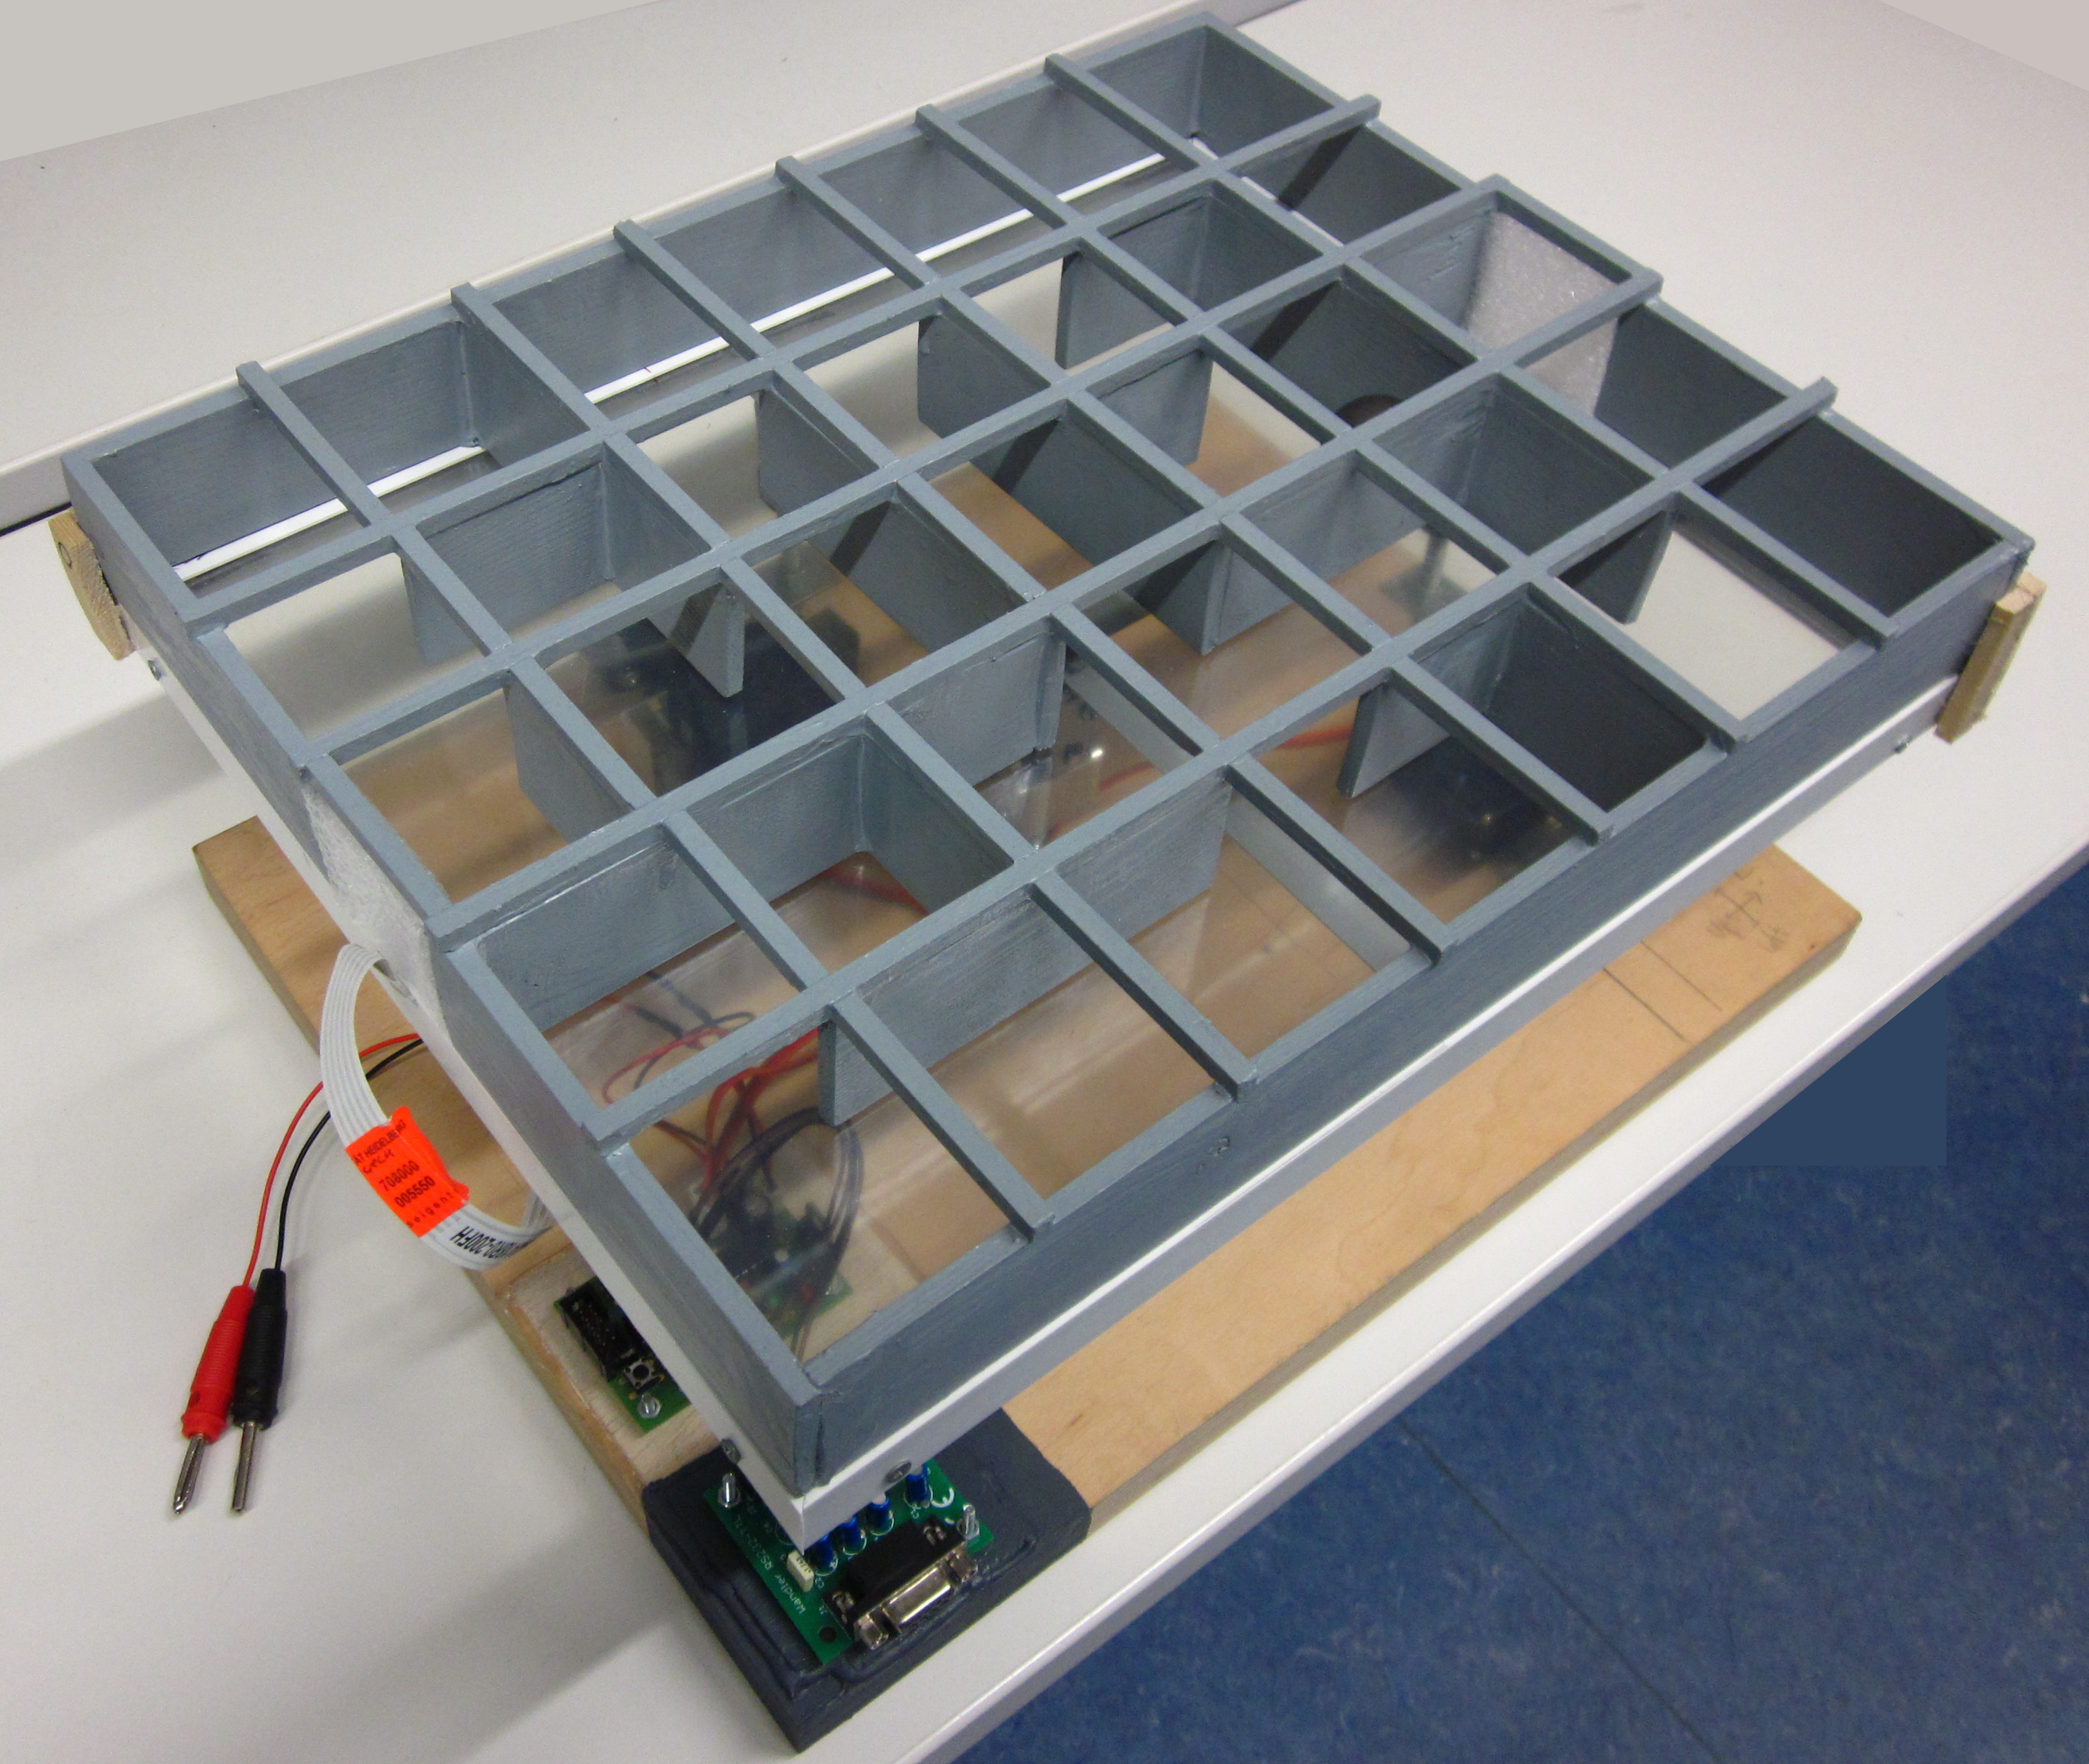
\includegraphics[scale=.2]{roboter_badly-photoshoped}
  %\caption{}
\end{figure}
\end{frame}

\begin{frame}[fragile,t]{Die \verb~Maze~-Klasse}{Datenstruktur für das Labyrinth}
\blue{\texttt{\longunderscore init\longunderscore (width, height)}}

\smallskip\noindent
Erstellt eine neue Instanz der \verb~Maze~-Klasse.

\medskip\noindent
\textbf{Beispiel:}

\medskip
\begin{minted}[bgcolor=black!85]{python}
m = Maze(5, 3)
print m

# Output:
#
# +--+--+--+--+--+
# |  |  |  |  |  |
# +--+--+--+--+--+
# |  |  |  |  |  |
# +--+--+--+--+--+
# |  |  |  |  |  |
# +--+--+--+--+--+
\end{minted}
\end{frame}

\begin{frame}[fragile,t]{Methoden der \verb~Maze~-Klasse}
\blue{\texttt{add\textunderscore edge(v1, v2)}}

\smallskip\noindent
Fügt eine Kante zwischen den Punkten \blue{\texttt{v1}} und \blue{\texttt{v2}}.

\medskip\noindent
\textbf{Beispiel:}

\medskip
\begin{minted}[bgcolor=black!85]{python}
m = Maze(5, 3)
m.add_edge((1, 1), (1, 2))
print m

# Output:
#
# +--+--+--+--+--+
# |  |  |  |  |  |
# +  +--+--+--+--+
# |  |  |  |  |  |
# +--+--+--+--+--+
# |  |  |  |  |  |
# +--+--+--+--+--+
\end{minted}
\end{frame}

\iffalse
\begin{frame}[fragile,t]{Methoden der \verb~Maze~-Klasse}
\blue{\texttt{add\textunderscore path(path)}}

\medskip\noindent
\textbf{Beispiel:}

\medskip
\begin{minted}[bgcolor=black!85]{python}
m = Maze(5, 3)
m.add_path([(1, 1), (1, 2), (2, 2), (3, 2), 
  (5, 3), (5, 2)])
print m

# Output:
#
# +--+--+--+--+--+
# |  |  |  |  |  |
# +  +--+--+--+--+
# |        |  |  |
# +--+--+--+--+  +
# |  |  |  |  |  |
# +--+--+--+--+--+
\end{minted}
\end{frame}

\begin{frame}[fragile,t]{Methoden der \verb~Maze~-Klasse}
\begin{itemize}
\item \blue{\texttt{has\textunderscore vertex(x, y)}}

\smallskip
Gibt ein \verb~bool~ zurück, ob sich der Punkt \blue{\texttt{(x, y)}} auf dem Graph befindet, oder nicht.
\item \blue{\texttt{has\textunderscore edge(v1, v2)}}

\smallskip
Gibt ein \verb~bool~ zurück, ob die Punkte \blue{\texttt{v1}} und \blue{\texttt{v2}} mit einer Kante verbunden sind, oder nicht.
\item \blue{\texttt{parse(string)}}

\smallskip
Liest die gegebene \verb~string~-Darstellung eines Labyrinths und fügt/entfernt Kanten, sodass das Objekt dieser Darstellung entspricht.
\end{itemize}
\end{frame}
\fi

\begin{frame}[fragile,t]{Methoden der \verb~Maze~-Klasse}
\begin{itemize}
\item \blue{\texttt{bfs(start, end)}}

\smallskip
Führt eine Breitensuche durch und gibt den kürzesten Pfad vom Punkt \blue{\texttt{start}} nach \blue{\texttt{end}} zurück.
\item \blue{\texttt{get\textunderscore neighbors(x, y)}}

\smallskip
Gibt eine Liste aller Punkten auf dem Graphen zurück, die genau Manhattan-Distanz 1 vom Punkt \blue{\texttt{(x, y)}} entfernt sind.
\item \blue{\texttt{get\textunderscore reachables(x, y)}}

\smallskip
Gibt eine Liste aller Punkten \verb~v~ in \verb~get_neighbors(x, y)~ zurück, die eine Kante nach \blue{\texttt{(x, y)}} haben.
\item \blue{\texttt{get\textunderscore skippables(path)}}
Gibt eine Liste aller Indizes \verb~i~ zurück, sodass \blue{\texttt{[path[i - 1], path[i], path[i + 1]]}} eine gerade Strecke bildet.
\end{itemize}
\end{frame}

\begin{frame}[fragile,t]{Kommunikationsmodell}
\begin{itemize}
\item Das Protokoll ist asymmetrisch
\begin{itemize}
\item Zwei Teilnehmer: MCU und \verb~Balancer~-Klasse
\end{itemize}
\item Der Kommunikationskanal wird als fehlerfrei angenommen
\item \verb~Balancer~ übergibt die Befehle, MCU antwortet
\end{itemize}
\end{frame}

\begin{frame}[fragile,t]{Kommunikationsmodell}{Antworten}
\begin{minted}{text}
[sign][x-coord],[y-coord]
\end{minted}

\begin{itemize}
\item Der MCU wird beim Balancieren der Kugel maximal 60 mal pro Sekunde eine Antwort senden.
\item \texttt{[x-coord]} und \texttt{[y-coord]} sind dreistellige Zahlen zwischen \texttt{025} und \texttt{555}, die die aktuellen Koordinaten der Kugel entspricht.
\item \texttt{[sign]} ist \texttt{=}, wenn die sich balanciert hat.
\item Ansonsten ist \texttt{[sign]} ein \texttt{:} (Doppelpunkt).
\end{itemize}
\end{frame}

\begin{frame}[fragile,t]{Kommunikationsmodell}{Befehle}
\begin{minted}{text}
[sign][x-coord],[y-coord]
\end{minted}

\begin{itemize}
\item Befehle können nur gesendet werden, wenn sich die Kugel balanciert hat.
\item \texttt{[x-coord]} und \texttt{[y-coord]} sind dreistellige Zahlen zwischen \texttt{025} und \texttt{555} und entsprechen die Koordinaten, die die Kugel ansteuern soll.
\item \texttt{[sign]} ist \texttt{!}, wenn die Servomotoren des Touchscreens auf den Anfangswerten zurückgesetzt werden sollen.
\item Ansonsten ist \texttt{[sign]} ein \texttt{.} (Punkt).
\end{itemize}
\end{frame}

\begin{frame}[fragile,t]{Die \verb~Balancer~-Klasse}{Kommunikation zwischen PC und MCU}

\blue{\texttt{\longunderscore init\longunderscore (serial, width=580, height=580, padding=25)}}

\smallskip\noindent
Erstellt eine neue Instanz der \verb~Balancer~-Klasse.\\
\blocking{Argumente mündlich erläutern!}

\medskip\noindent
\textbf{Beispiel:}

\medskip
\begin{minted}[bgcolor=black!85]{python}
def balanced(destination, response, reached):
    if reached: return
    balancer.add_command(290, 290)

balancer = Balancer(serial.Serial(0))
balancer.balance_handler = balanced
balancer.add_command(290, 290)
balancer.start_listening()
balancer.serial.close()
\end{minted}
\end{frame}

\begin{frame}[fragile,t]{Ablauf der Wanderkennung}{Anfangssequenz}
\begin{small}
\begin{figure}[h]
  \centering
  \begin{tikzpicture}
	\node at (0, 0) [startend] (start) {Start};
	\node at (0, -1.75) [block, text width=3cm] (nstack) {Generiere \verb~neighbors_stack~ von \verb~anchor~};
	\node at (0, -3.75) [block, text width=3cm] (init) {Initialisierung: Balanciere Kugel auf \verb~anchor~ aus};
	\node at (0, -5.5) [kugel] (kugel) {Kugel ist ausbalanciert};
	\path [line] (start) -- (nstack);
	\path [line] (nstack) -- (init);
	\path [line] (init) -- (kugel);
  \end{tikzpicture}
\end{figure}
\end{small}
\end{frame}

\begin{frame}[fragile,t]{Ablauf der Wanderkennung}{Die Kugel hat ihr Ziel erreicht}
\begin{tiny}
\begin{figure}[h]
  \centering
  \begin{tikzpicture}
	\node at (0, 0) [kugel, text width=1.25cm] (kugelstart) {Kugel ist ausbalanciert};
	\node at (0, -3) [startend] (ende) {Ende};
	\node at (3, 0) [decision, text width=1.25cm] (amziel) {Ist die Kugel am Ziel?};
	\node at (3, -3) [decision, text width=1.75cm] (stackleer) {Ist \verb~neighbors_stack~ leer?};
	\node at (6, -1) [block, text width=1.25cm] (erreichbar) {$n$ ist\\ erreichbar};
	\node at (6, -3) [decision, text width=1.25cm] (istnachbar) {Ist Ziel ein Nachbar $n$?};
	\node at (6, 0) [block, text width=1.25cm] (gehezurueck) {Gehe zurück zu \verb~anchor~};
	\node at (9, 0) [kugel, text width=1.25cm] (kugelende) {Kugel ist ausbalanciert};
	\node at (9, -3) [block, text width=1.75cm] (weiter) {Hole einen (neuen) Nachbarn $n$ aus \verb~neighbors_stack~ und schicke die Kugel dorthin};
	\path[line] (kugelstart) -- (amziel);
	\path[line] (amziel) -- node[left]{J} (stackleer);
	\path[line] (stackleer) -- node[above]{J} (ende);
	\path[line] (stackleer) -- node[above]{N} (istnachbar);
	\path[line] (istnachbar) -- node[left]{J} (erreichbar);
	\path[line] (erreichbar) -- (gehezurueck);
	\path[line] (gehezurueck) -- (kugelende);
	\path[line] (istnachbar) -- node[above]{N} (weiter);
	\path[line] (weiter) -- (kugelende);
	\draw[thick, dashed, draw=blue!50!black!70] (kugelende) -- (9, 1.25) -- (0, 1.25) -- (kugelstart);
	\draw[thick, gray, ->] (amziel) -- node[left]{N} (3, 2);	
  \end{tikzpicture}
\end{figure}
\end{tiny}
\end{frame}

\begin{frame}[fragile,t]{Ablauf der Wanderkennung}{Die Kugel hat ihr Ziel nicht erreicht}
\begin{tiny}
\begin{figure}[h]
  \centering
  \begin{tikzpicture}
	\node at (0, 0) [kugel, text width=1.25cm] (kugelstart) {Kugel ist ausbalanciert};
	\node at (0, 3) [block, text width=1.25cm] (versucheerneut) {Versuche es erneut};
	\node at (3, 0) [decision, text width=1.25cm] (amziel) {Ist die Kugel am Ziel?};
	\node at (3, 3) [decision, text width=1.25cm] (istanchor) {Ist \verb~anchor~ das Ziel?};
	\node at (6, 3) [decision, text width=1.25cm] (zweimal) {Bereits zweimal versucht?};
	\node at (6, 1) [block, text width=1.25cm] (wand) {Zwischen \verb~anchor~ und Nachbarn $n$};
	\node at (6, 0) [block, text width=1.25cm] (setzezurueck) {Setze die\\ Servomotoren zurück};
	\node at (9, 0) [kugel, text width=1.25cm] (kugelende) {Kugel ist ausbalanciert};
	\path[line] (kugelstart) -- (amziel);
	\draw[thick, dashed, draw=blue!50!black!70] (kugelende) -- (9, -1.25) -- (0, -1.25) -- (kugelstart);
	\path[line] (amziel) -- node[left]{N} (istanchor);
	\path[line] (istanchor) -- node[above]{J} (versucheerneut);
	\path[line] (versucheerneut) -- (kugelstart);
	\path[line] (istanchor) -- node[above]{N} (zweimal);
	\path[line] (zweimal) -- (6, 4.25) -- node[above]{N} (0, 4.25) -- (versucheerneut);
	\path[line] (zweimal) --  node[left]{J} (wand);
	\path[line] (wand) -- (setzezurueck);
	\path[line] (setzezurueck) -- (kugelende);
	\draw[thick, gray, ->] (amziel) -- node[left]{J} (3, -2);
  \end{tikzpicture}
\end{figure}
\end{tiny}
\end{frame}

\begin{frame}[fragile,t]{Optimierung}
\begin{itemize}
\item Die Funktion \verb~run(path, maze)~ berücksichtigt durch \verb~maze.get_skippables(path)~ erhaltene Felder
\item \verb~detect_walls~ lässt die Kugel auf dem letzten Nachbarn, falls dieser erreichbar war
\begin{itemize}
\item Erspart unnötiges Zurückgehen zum Anker
\end{itemize}
\item \verb~detect_maze~ berücksichtigt das letzte Ziel der Kugel 
\begin{itemize}
\item Falls die Kugel auf einem Nachbarn gelassen wurde wird dieser zum neuen Anker für \verb~detect_walls~ gemacht 
\end{itemize}
\end{itemize}
\end{frame}

\begin{frame}[fragile,t]{Aufgetretene Probleme}
%Durch den unempfindlichen inneren Rand des Touchscreens dauert das Ausbalancieren in Randnähe durchschnittlich länger. Auch in verhältnismäßig kleinen Labyrinthfeldern können Verzögerungen bei der Erkennung des Labyrinths auftreten. Die naheliegende Lösung beider Probleme ist eine Verbesserung der Hardware.
\textbf{Problem:}\\
Das \blue{Ausbalancieren im Toleranzbereich} einzelner Felder \blue{dauert gelegentlich verhältnismäßig lange}

\medskip\noindent
\textbf{Gründe:}
\begin{itemize}
\item Der unempfindliche Rand des Touchscreens
\item Unterschiede in der Größe der Felder des realen Labyrinths
\end{itemize}

\medskip\noindent
\textbf{Folgen:} \blue{Verzögerungen bei} der \blue{Erkennung des Labyrinths}

\medskip\noindent
\textbf{Lösungsansätze:}
\begin{itemize}
\item Toleranzbereich kurzzeitig vergrößern
\textcolor{gray}{
\item[\textcolor{gray}{$\triangleright$}] Hardware verbessern
}
\end{itemize}
\end{frame}

\begin{frame}[fragile,t]{Ausblick/Reflexion}
Das Praktikum hat uns sehr gefallen und war ein guter Ausgleich zu unseren Vorlesungen.

\medskip\noindent
Wir denken nicht, dass sich der Roboter (bezogen auf unsere Aufgabenstellung) wesentlich verbessern lässt. Mögliche Erweiterungen:
\begin{itemize}
\item Labyrinthmaße experimentell bestimmen lassen
\item GUI schreiben
\textcolor{gray}{
\item[\textcolor{gray}{$\triangleright$}] Hardware erneuern und optimieren (beinhaltet Arbeit am MCU-Code)
}
\end{itemize}
\end{frame}


%\begin{frame}[fragile,t]{Thema}{Unterthema}
%\verb~print('Hello world!')~
%\end{frame}

\end{document}
